\chapter{Marco teórico: Autómatas celulares}
\label{chapter:automatas_celulares}

La investigación de los sistemas complejos es un reto actual de la ciencia moderna. Estos sistemas, caracterizados por la interacción entre múltiples componentes locales, son capaces de generar comportamientos emergentes y, a veces, caóticos. Para entender esta complejidad necesitamos herramientas que puedan capturar la esencia de la autoorganización, y aquí los autómatas celulares surgen como un modelo computacional clave para simular fenómenos tanto naturales como artificiales.

En este capítulo se definen los fundamentos matemáticos y estructurales de un autómata celular. Este se entiende como un sistema dinámico discreto, que combina un conjunto de celdas interconectadas y que pueden producir patrones complejos a partir de reglas locales. Se mencionarán sus elementos esenciales, tales como:

\begin{itemize}
	
	\item El vecindario: El subconjunto de celdas que afecta el cambio de una unidad.
	
	\item El estado de conjunto: Los valores finitos que puede tomar cada celda.
	
	\item Las condiciones de frontera son: El comportamiento del sistema en sus límites en el espacio.
	
	\item Las funciones de transición son: El algoritmo que rige la evolución del sistema.
	
\end{itemize}

Se revisan, asimismo, ejemplos que han sido de una importancia capital para el desarrollo de esta disciplina, tales como el Juego de la Vida de John Conway y los autómatas celulares elementales de Stephen Wolfram.

Finalmente, el capítulo amplía la definición clásica hacia terrenos más avanzados. Se presentan autómatas celulares que operan en espacios no euclidianos y se examinan extensiones recientes que incluyen estados continuos, reglas de probabilidad o actualizaciones asíncronas. Estas variaciones hacen que los AC continúen siendo, décadas después de ser concebidos por Von Neumann, una herramienta de vanguardia en campos tan diversos como la biología teórica, la criptografía y la física de partículas.

\section{Autómata celular}

Los autómatas celulares, concebidos por John von Neumann en 1948 \cite{damerow2010_neumann}, son una colección de células donde cada una de ellas puede adquirir un estado y se agrupan en una red. Además, estas células evolucionan en intervalos y cada una de ellas actualiza su estado en función del estado de sus células vecinas \cite{weisstein2002_ca, wolfram1982_ca, fsancho2016_ca}. 

Siguiendo de manera general a \cite{bhattacharjee2019_ca, sayama2024_ca, Ilachinski2001_ca}, y considerando una red regular de células, un conjunto finito de estados y evoluciones en pasos discretos de tiempo, se define a un autómata celular como:

\begin{definition}
	Un autómata celular es una 4-tupla ($\mathcal{L}, \mathcal{S}, \mathcal{N}, \mathcal{R}$) donde:
	\begin{itemize}
		\item $\mathcal{L} \subseteq \mathbb{Z}^D$ es el espacio celular $D$-dimensional. El conjunto de células vive en el espacio $\mathcal{L}$ y cada célula $\vec{i}$ se define como un vector $D$-dimensional que representa su posición en el espacio.
		
		\item $\mathcal{S}$ es un conjunto de $k$ estados. Cada célula $\vec{i}$ solo puede adquirir un valor de un conjunto finito de diferentes estados:	
		\[
		\sigma_{\vec{i}}(t) \in \mathcal{S} \equiv \{ s_0, s_1,s_2, \dots, s_{k - 1} \},\; \forall \vec{i} \in \mathcal{L}
		\]
		Donde $\vec{i} \in \mathcal{L}$ es una célula en el espacio celular, $\sigma_{\vec{i}} (t)$ es el estado de la i-ésima célula en el tiempo $t$ y $\mathcal{S}$ es un anillo conmutativo finito, como un intervalo de números enteros, que generalmente se define por los enteros módulo $k$ ($\mathbb{Z}_k$).
			
		\item $\mathcal{N} = (\vec{v}_1, \vec{v}_2, \dots, \vec{v}_m )$ es el conjunto de los $m$ vectores de desplazamiento que definen la vecindad de una célula en $\mathcal{L}$. Así, los vecinos de las células ubicadas en $\vec{i} \in \mathcal{L}$ se encuentran en las posiciones $\vec{i} + \vec{v}, \forall \vec{v} \in \mathcal{N}$ 
		
		\item $\mathcal{R} : \mathcal{S}^m \to \mathcal{S}$ es la regla local del autómata:
		\[
		\sigma_{\vec{i}}(t + 1) = \mathcal{R} ( \{ \sigma_{\vec{i} + \vec{v}_j}\}_{j = 1}^m  )
		\]
		donde $\mathcal{R}$ es la función de transición local que asigna el nuevo estado de una célula a partir de los estados de sus $m$ vecinos.		
	\end{itemize}
	
\end{definition}

\section{Vecindad}

Como ya se mencionó, la vecindad es el conjunto de vectores de desplazamiento, por lo que está estrechamente relacionado con la dimensionalidad del autómata celular. Por ejemplo, John von Neumann propuso una vecindad para $\mathbb{Z}^2$ de cinco células que actualmente se conoce como vecindad de von Neumann. Esta vecindad considera a la célula y a sus cuatro vecinas ortogonales más cercanas \cite{neumann1966_ca}, dicho de otro modo:
\[
	\mathcal{N} = ((0, -1), (-1, 0), (0, 0), (1, 0), (0, 1))
\]
La cual se puede representar como en la figura \ref{fig:N_neumann}. 

Por otro lado, Moore añade los cuatro vecinos diagonales más cercanos a la vecindad de von Neumann, dando una vecindad de nueve elementos \cite{Kwon2015_moore}. Esta vecindad, representada por la figura \ref{fig:N_moore}, fue utilizada por John Conway en el ``Juego de la Vida'' \cite{lifewiki_life}.

Otro ejemplo se encuentra en la figura \ref{fig:N_wolfram}, la cual representa una vecindad de radio uno en un espacio unidimensional, es decir, todas aquellas células a una distancia menor o igual a uno, incluyéndose a su misma. Fue utilizada por Stephen Wolfram para definir los autómatas celulares elementales \cite{Wolfram2002_nks}.

\begin{figure}[!htbp]
	\centering
	\begin{subfigure}[b]{0.30\textwidth}
		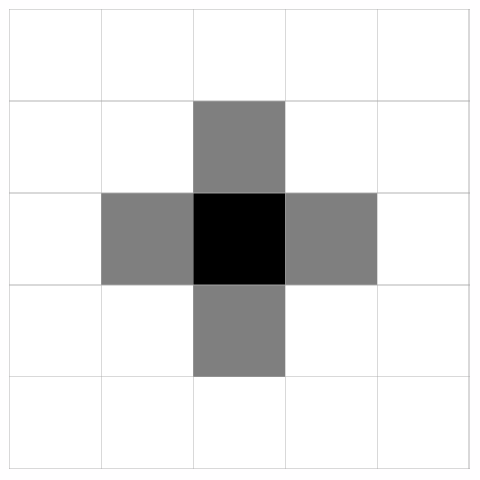
\includegraphics[width=\textwidth]{img/nNeumann.png}
		\caption{Vecindad de von Neumann}
		\label{fig:N_neumann}
	\end{subfigure}
	\begin{subfigure}[b]{0.30\textwidth}
		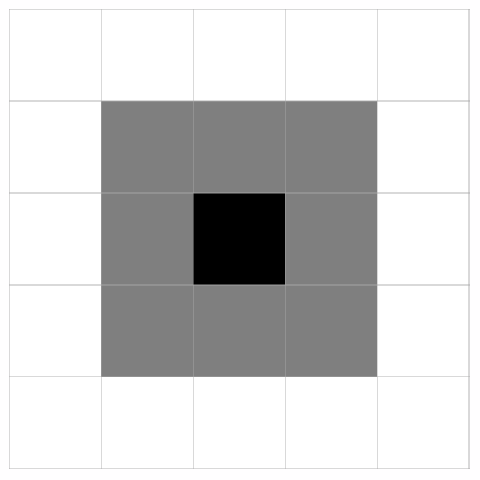
\includegraphics[width=\textwidth]{img/nMoore.png}
		\caption{Vecindad de Moore}
		\label{fig:N_moore}
	\end{subfigure}
	\begin{subfigure}[b]{0.40\textwidth}
		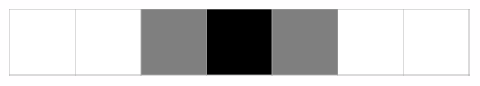
\includegraphics[width=\textwidth]{img/nWolfram.png}
		\caption{Vecindad de radio uno en $\mathbb{Z}^1$}
		\label{fig:N_wolfram}
	\end{subfigure}
	\caption{Las vecindades \ref{fig:N_neumann} y \ref{fig:N_moore} son para CA bidimensionales; la \ref{fig:N_wolfram} es para CA unidimensionales. La célula negra representa la célula actual y, junto con las grises, conforma su vecindad.}
	
	\label{fig:vecindades_regulares}
	
\end{figure}

Las vecindades no solo son cuadradas; también pueden tener otras formas, como hexágonos o triángulos, que se muestran en las figuras \ref{fig:N_hexagonal} y \ref{fig:N_triangular}.  Además, existen vecindades con comportamiento dinámico, como la de Margolus mostrada en la figura \ref{fig:N_margolus}, cuya configuración alterna entre dos disposiciones en cada paso evolutivo \cite{tyler2018_margolus}.

\begin{figure}[!htbp]
	\centering
	\begin{subfigure}[b]{0.30\textwidth}
		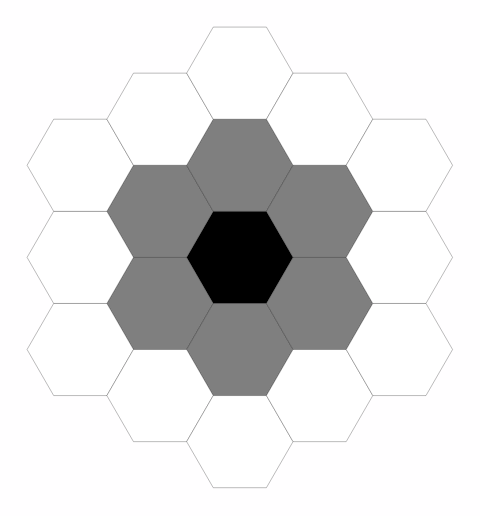
\includegraphics[width=\textwidth]{img/nHexagon.png}
		\caption{Vecindad hexagonal}
		\label{fig:N_hexagonal}
	\end{subfigure}
	\begin{subfigure}[b]{0.30\textwidth}
		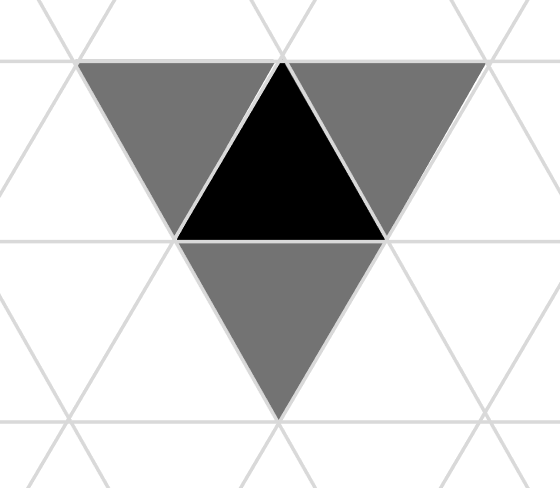
\includegraphics[width=\textwidth]{img/nTriangular.png}
		\caption{Vecindad triangular}
		\label{fig:N_triangular}
	\end{subfigure}
	\begin{subfigure}[b]{0.30\textwidth}
			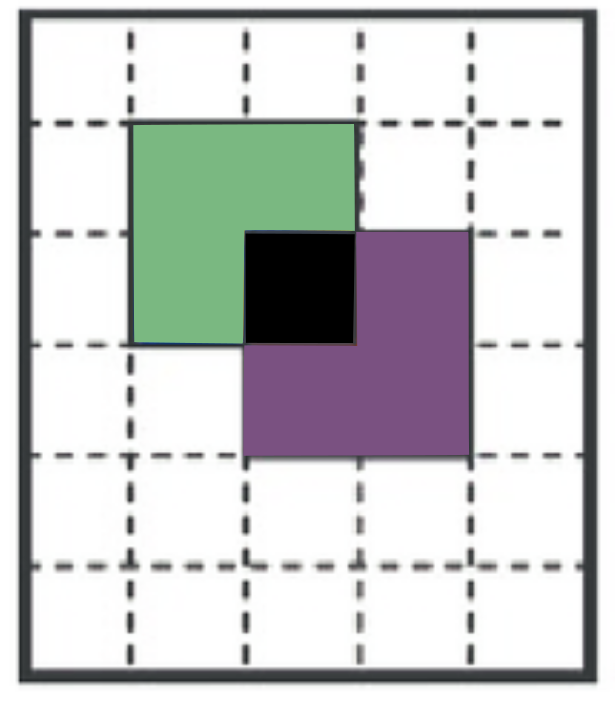
\includegraphics[width=\textwidth]{img/nMargolus.png}
		\caption{Vecindad de Margolus}
		\label{fig:N_margolus}
	\end{subfigure}
	
	\caption{En \ref{fig:N_hexagonal} y \ref{fig:N_triangular}, la célula negra es la actual y las grises su vecindad.  En \ref{fig:N_margolus}, la célula negra es la actual, mientras que las células verdes y moradas representan las vecindades activas en tiempos pares e impares.}
	
	\label{fig:vecindades_irregulares}
	
\end{figure}

Finalmente, los vecinos no tienen que ser estrictamente adyacentes entre sí ni ser simétricos. Existen vecindades, como en la figura \ref{fig:N_noadyacente}, donde algunas células no son contiguas a la central.

\begin{figure}[!htbp]
	\centering
	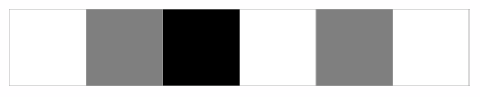
\includegraphics[width=0.5\textwidth]{img/nNoAdyacente.png}
	\caption{Vecindad en $\mathbb{Z}^1$ con vecinos de adyacentes.}
	\label{fig:N_noadyacente}
\end{figure}

\section{Estados}

Cada célula adquiere un único estado $s$ en cada paso de tiempo, donde $s$ pertenece a un conjunto de estados $s \in \mathcal{S}$. Por ejemplo, el autómata celular de John von Neumann contempla 29 estados, aunque algunos autores han propuesto variantes reducidas a cuatro estados, conservando su capacidad de autoreproducirse \cite{bhattacharjee2019_ca}. 

Por otro lado, el juego de la vida se compone de dos estados que denominó ``vivas'' y ``muertas'' \cite{lifewiki_life}.  De igual forma, Stephen Wolfram utiliza dos estados en los autómatas celulares elementales \cite{Wolfram2002_nks}.

Idealmente, el espacio celular $\mathcal{L}$ es infinito, lo que permitiría infinitas combinaciones de estados. Sin embargo, esto es inviable computacionalmente. Para esto, se requiere establecer una restricción de finitud, como lo marca \cite{bhattacharjee2019_ca}.
 
 Supóngase un espacio discreto unidimensional infinito. Idealmente, conocemos el estado de las infinitas células, pero computacionalmente no podemos almacenar ni procesar toda esa información. Por lo que se restringe a los valores que únicamente nos interesan. 
 
 A todas aquellas células que son de interés se les define con un estado activo, el cual puede ser cualquier $s \in \mathcal{S}$, por otro lado, las que no son de interés se les define con un estado inactivo $\sigma_q$:
 
\begin{definition}
	Sea $\mathcal{R}$ la regla local de un autómata celular. Un estado $\sigma_q \in \mathcal{S}$ es inactivo si $\mathcal{R}(\sigma_q, \sigma_q, \dots, \sigma_q) = \sigma_q$.
	\label{def:estado_inactivo}
\end{definition}

Es decir, si una célula y todos sus vecinos están en estado inactivo, la célula permanece inactiva tras aplicar $\mathcal{R}$. Cabe notar que todos los vecinos deben estar en dicho estado, por lo que, si alguno cambia a cualquier estado $s$, entonces se  activa. Este evento ocurre cuando el espacio en donde evoluciona el autómata celular incrementa. 

Para trabajar computacionalmente, \cite{bhattacharjee2019_ca} define las configuraciones finitas de la siguiente manera:

\begin{definition}	
	Sea $\sigma_q \in \mathcal{S}$ un estado inactivo, $\sigma_p \neq \sigma_q \in \mathcal{S}$ un estado no inactivo y sea $\mathcal{L}$ un espacio celular infinito. Se considera que un autómata celular tiene configuración finita si solo un número finito de celdas están en estados activos $\sigma_p$.
\end{definition}

Si la configuración inicial es finita, la propiedad de finitud se preserva en cada paso de tiempo, como se observa en la tabla \ref{tab:CA_finito}. Imaginemos un autómata celular en $\mathbb{Z}^1$ con una vecindad de radio 1 y una sola célula activa en la posición $n$ con estado $\sigma_p$, mientras que el resto de infinitas células tienen estado inactivo $\sigma_q$. 

En el tiempo $t + 1$ las células en $n - 1$ y en $n + 1$ tienen un vecino que no es inactivo, por lo que pasan a ser activas por la definición \ref{def:estado_inactivo}. Dado que este incremento está acotado por el tamaño de la vecindad, la configuración resultante sigue siendo finita. Por inducción, este proceso se repite para cualquier tiempo $t + m$; por lo tanto, mientras el tiempo de la evolución no tienda a infinito ($t \not\to \infty $) el autómata celular mantendrá una configuración finita, garantizando su viabilidad computacional.

\begin{table}
	\centering
	\begin{tabular}{c | c c c c c c c c c c c} 
		$t$ & \multicolumn{11}{c}{ $\vec{\sigma}(t)$  } \\ \hline \hline
		0 & && & \dots & $q$ & $p$ & $q$ & \dots & && \\ \hline
		1 & & & \dots & $q$ & $p$ & $p$&  $p$ & $q$ & \dots & & \\ \hline
		2  & & \dots & $q$  & $p$ & $p$ & $p$&  $p$ &  $p$& $q$ & \dots &  \\ \hline
		3 & \dots & $q$  & $p$ & $p$ & $p$&  $p$&$p$ &$p$& $p$ & $q$ & \dots \\
	\end{tabular}
	\caption{Evolución temporal de un autómata celular unidimensional con una configuración inicial finita. Donde $p$ representa estados activos y $q$ estados inactivos. Los conjuntos $\vec{\sigma} (t)$ y $\vec{\sigma} (t + n)$ son finitos.}
	\label{tab:CA_finito}
\end{table}

Sea $\mathcal{C} =  \mathcal{S}^\mathcal{L}$ el conjunto de todas las configuraciones. Definimos $\mathcal{C}_F \subset \mathcal{C}$ como el subconjunto de todas las configuraciones finitas. Esta restricción es necesaria para hacer computacionalmente viable la simulación de la evolución.

\begin{comment}
	Finalmente, resulta necesario definir un estado estable, el cual servirá más adelante para establecer una clasificación \cite{bhattacharjee2019_ca}. 

\begin{definition}
	
	Dado un autómata celular y un estado $s \in \mathcal{S}$, se dice que $s$ es un estado estable si $\mathcal{R}(s, s, \dots, s) = s$.
	
\end{definition}

Esto es, un estado estable $s$ que evoluciona siempre en sí mismo, por lo que $\sigma(t) = \sigma(t + 1)$. 
\end{comment}

\section{Condiciones de frontera}

Idealmente, los autómatas celulares pueden evolucionar en espacios infinitos; sin embargo, se pueden establecer límites o fronteras, las cuales restringen el espacio celular $\mathcal{L}$ \cite{bhattacharjee2019_ca, ponce2015_ca}.

\begin{definition}
	Un autómata celular es finito si el espacio celular $\mathcal{L} \subseteq \mathbb{Z}^D$ es finito; en caso contrario, se denomina infinito. 
\end{definition}

Un autómata celular finito siempre tiene fronteras en los límites de su espacio. A la forma en como se comporta la frontera se le conoce como condición de frontera, la cual suele ser abierta o periódica \cite{ponce2015_ca}.

\begin{itemize}
	\item \textbf{Condición de frontera abierta}: Se les asigna un estado fijo a todos aquellos vecinos faltantes en las células de la frontera. 
	\item \textbf{Condición de frontera periódica}: Los vecinos faltantes de las células en la frontera son otras células en la frontera. La figura \ref{fig:B_periodica} muestra cómo se conectan las células de la frontera en un espacio unidimensional.
\end{itemize}

\begin{figure}[!htbp]
	\centering
	\begin{subfigure}[b]{0.45\textwidth}
		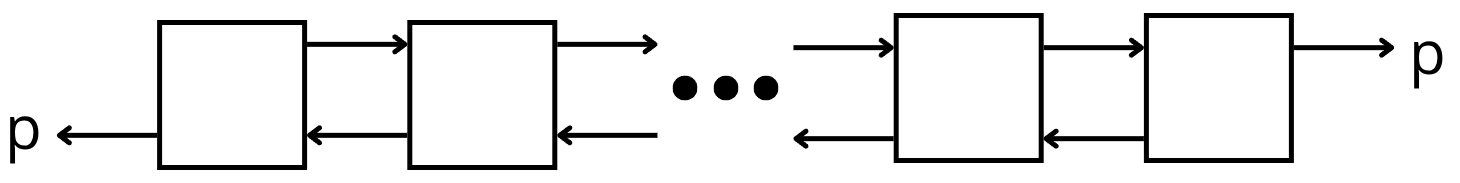
\includegraphics[width=\textwidth]{img/bAbierta.png}
		\caption{Condición de frontera abierta}
		\label{fig:B_abierta}
	\end{subfigure}
	\begin{subfigure}[b]{0.45\textwidth}
		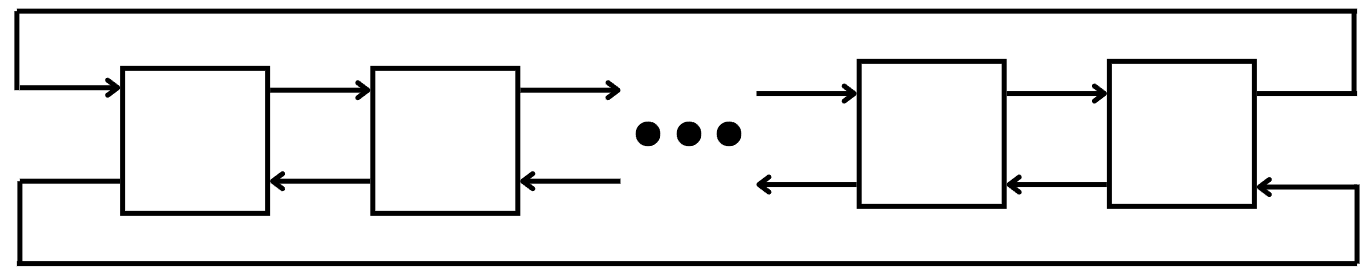
\includegraphics[width=\textwidth]{img/bPeriodica.png}
		\caption{Condición de frontera periódica}
		\label{fig:B_periodica}
	\end{subfigure}
	
	\caption{Condiciones de frontera con dos vecinos. La figura \ref{fig:B_abierta} asigna un estado no inactivo al vecino faltante. La figura \ref{fig:B_periodica} asigna como vecino el estado de la célula en la frontera opuesta, formando un anillo.}
	
	\label{fig:fronteras}
	
\end{figure}

Un autómata infinito que tiene una configuración periódica equivale a un autómata finito con frontera periódica \cite{bhattacharjee2019_ca}.

\begin{definition}
	Una configuración $\vec{\sigma} \in \mathcal{C}$ de un autómata celular $D$-dimensional se dice periódica si es invariante ante un conjunto de traslaciones linealmente independientes en $D$ direcciones. Es decir:
	\[
	\vec{\sigma} = T_i^{n_i} (\vec{\sigma}), \; \forall i \in \{ 1,2, \dots, D \}
	\]
	donde  $T_i^{n_i}$ denota un desplazamiento de $n_i$ posiciones en la dimensión $i$.
\end{definition}

Definimos entonces a $\mathcal{C}_P \subset \mathcal{C}$ como el conjunto de todas las configuraciones periódicas. Estas configuraciones preservan la condición de frontera periódica en cada traslación \cite{bhattacharjee2019_ca}. 

La frontera no solo puede ser abierta o periódica, existen diferentes comportamientos como la reflectiva y la reflexiva. La frontera reflectiva asigna a los vecinos faltantes el mismo estado de la célula en la frontera (figura \ref{fig:B_reflectiva}), por lo que son vecinas de si mismas. La frontera reflexiva, en cambio, genera una doble relación de vecindad en los extremos (figura \ref{fig:B_reflexiva}), \cite{bhattacharjee2019_ca, ponce2015_ca}.

\begin{figure}[!htbp]
	\centering
	\begin{subfigure}[b]{0.45\textwidth}
		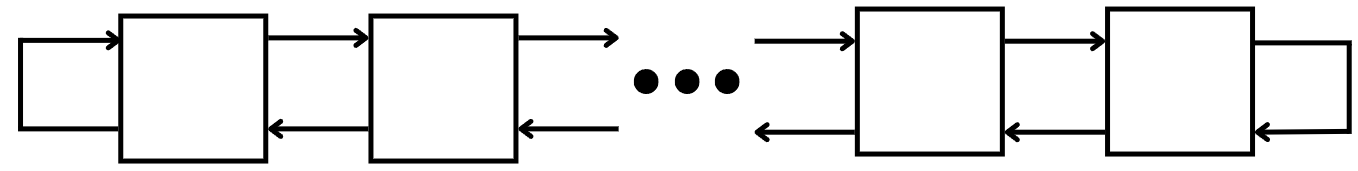
\includegraphics[width=\textwidth]{img/bReflectiva.png}
		\caption{Condición de frontera reflectiva}
		\label{fig:B_reflectiva}
	\end{subfigure}
	\begin{subfigure}[b]{0.45\textwidth}
		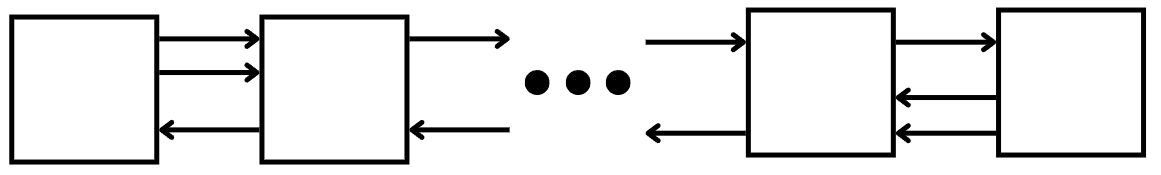
\includegraphics[width=\textwidth]{img/bReflexiva.png}
		\caption{Condición de frontera reflexiva}
		\label{fig:B_reflexiva}
	\end{subfigure}
	
	\caption{Condiciones de frontera con dos vecinos. La figura \ref{fig:B_reflectiva} muestra que las células en la frontera son vecinas entre sí, mientras que la figura \ref{fig:B_reflexiva} indica que las células que están al lado de las células de la frontera pueden tener múltiples relaciones de vecindad.}
	\label{fig:fronteras_adicionales}
\end{figure}

\section{Regla local}

Sea $\mathcal{S}$ el conjunto de estados y $m = |\mathcal{N}|$ el número de vecinos. La función de transición o regla local se define como 
\[
\mathcal{R}: \mathcal{S}^m \to \mathcal{S}
\] 
donde $\mathcal{R}$ asigna un nuevo estado a cada célula en función de los estados de sus $m$ vecinos (incluyéndose a sí misma si aplica).

Para autómatas celulares unidimensionales, dado un rango arbitrario $r$, la regla puede ser escrita como:
\[
\sigma_{i}(t + 1) = \mathcal{R}(\sigma_{i-r}(t), \sigma_{i-r+1} (t), \dots, \sigma_{i}(t), \dots, \sigma_{i+r} (t)), \; \mathcal{R}:  S^{2r + 1} \to S
\]
Donde el radio $r$ especifica el tamaño de la vecindad para cada célula (la vecindad es de tamaño $2r + 1$ como se muestra en la figura \ref{fig:N_wolfram}), la cual puede adquirir un valor $k$.

Un ejemplo de regla local es el juego de la vida \cite{lifewiki_life}. En este caso, el conjunto de estados es binario $\mathcal{S} = \{ 0, 1 \}$, donde $0$ representa células muertas y $1$ las vivas. La regla de transición realiza el siguiente mapeo:
\[
\mathcal{R}: \{ 0, 1 \}^9 \to \{ 0, 1\}
\]
Ya que la vecindad de Moore en 2D involucra 8 vecinos más la propia célula, es decir, $m = 9$. 

El juego de la vida sigue las siguientes tres reglas:

\begin{itemize}
	
	\item \textbf{Nacimiento}: Una célula muerta en el tiempo $t$ nace en el tiempo $t + 1$ si tiene exactamente tres vecinos vivos en el tiempo $t$.
	\item \textbf{Muerte}: Una célula viva en el tiempo $t$ muere en $t + 1$ por:
	\begin{itemize}
		\item Sobrepoblación; si hay más de tres vecinos vivos en $t$.
		\item Soledad: si hay menos de dos vecinos vivos en $t$.
	\end{itemize}
	\item \textbf{Supervivencia}: Una célula viva en el tiempo $t$ se mantiene viva en $t + 1$ si tiene dos o tres vecinos vivos en $t$.	 
\end{itemize}

Esta se conoce como regla semitotalística, ya que la transición depende de la suma de los valores en la vecindad, pero distingue entre diferentes posiciones, como el centro y los bordes \cite{genaro2022_semitotalistic}.

Por otro lado, una regla es totalística si la transición depende únicamente de la suma de los estados en todos los vecinos, sin distinguir posiciones \cite{weisstein2002_totalistic}. Para un autómata celular unidimensional con $|\mathcal{S}| = 3$ estados y radio $r = 1$, solo hay $(|\mathcal{S}|-1) |\mathcal{N}|+1 = (2-1) \cdot 3 + 1 = 4$ posibles valores de suma.

Finalmente, una regla local es arbitraria si distingue las posiciones de cada elemento en la vecindad. Cabe mencionar que las reglas arbitrarias contienen todas las posibles combinaciones de reglas, incluyendo las semitotalísticas, las cuales incluyen a su vez las totalísticas:
\[
	\mathcal{R}_{\text{totalísticas}} \subset \mathcal{R}_{\text{semitotalísticas}} \subset \mathcal{R}_{\text{arbitrarias}}
\]
El objetivo de las reglas semitotalísticas y totalísticas será entonces simplificar ciertos comportamientos.

La configuración dada para el autómata celular elemental considera $k = 2$ (es decir, $\sigma_i \in \{0, 1\}$), un radio $r = 1$ ($|\mathcal{N}| = 3$) y la regla $\mathcal{R}: \{0,1\}^3 \rightarrow \{0,1\}$ que se define como:
\[
\phi(\sigma_{i-1}(t), \sigma_{i}(t), \sigma_{i+1}(t))
\]
Esta dinámica está dada por las posibles configuraciones que las tres células adyacentes pueden adquirir en el tiempo $t$. Podemos encontrar $k^{|\mathcal{N}|} = 2^3 = 8$ patrones posibles en la vecindad, número correspondiente a la combinatoria de dos estados en tres posiciones. Cada vez que encontremos un patrón, podemos asignarle un nuevo estado a $\sigma_i(t + 1)$ ($\{ 0, 1 \}$), por lo que el número total de reglas asciende a $k^{k^{|\mathcal{N}|}} = 2^8 = 256$, como se muestra en la tabla \ref{tab:ECA_evolucion}.

\begin{table}
	
	\centering
	
	\begin{tabular}{c c c c c c c c} 
		
		111 & 110 & 101 & 100 & 011 & 010 & 001 & 000 \\
		
		$\downarrow$ & $\downarrow$ & $\downarrow$ & $\downarrow$ & $\downarrow$ & $\downarrow$ & $\downarrow$ & $\downarrow$ \\
		
		$\{ 0, 1 \}$ & $\{ 0, 1 \}$ & $\{ 0, 1 \}$ & $\{ 0, 1 \}$ & $\{ 0, 1 \}$ & $\{ 0, 1 \}$ & $\{ 0, 1 \}$ & $\{ 0, 1 \}$ 
		
	\end{tabular}
	
	\caption{Cada posible combinación de tres células puede adquirir uno de dos valores. Cuando la célula evaluada encaja en este patrón, su valor cambia al establecido por la regla. Este conjunto de 256 reglas se le conoce como autómata celular elemental.}
	
	\label{tab:ECA_evolucion}
	
\end{table}

Estas reglas se pueden representar de forma tabular y también como un número decimal. La tabla \ref{tab:ECA_rules} muestra la asociación entre la forma tabular y la regla decimal.

Nótese que la regla decimal solo aplica cuando las condiciones son las mismas. Es decir, cuando el número de vecinos $|\mathcal{N}|$ y estados $|\mathcal{S}|$ son invariantes; a cada regla se le puede asociar un entero único, pero dos reglas que difieren en vecindad o estados pueden compartir el número decimal. Por ejemplo, considerando la regla $10$ con $|\mathcal{N}| = 2$ y $|\mathcal{S}| = 2$ es $1010$, la cual es completamente diferente cuando $|\mathcal{N}| = 3$ y $|S| = 2$, lo que da como resultado $ 000000101$.

\begin{table}
	
	\centering
	
	\begin{tabular}{c | c c c c c c c c | c} 
		
		\textbf{Binario} &111 & 110 & 101 & 100 & 011 & 010 & 001 & 000 & \multirow{3}{*}{\textbf{regla}} \\ 
		
		\textbf{Decimal} & 7 & 6 & 5 & 4 & 3 & 2 & 1 & 0 & \\ 
		
		\textbf{Valor} & $2^7$ & $2^6$ & $2^5$ & $2^4$ & $2^3$ & $2^2$ & $2^1$ & $2^0$ & \\ \hline
		
		& 0 &  0 &  0 &  0 &  0 &  0 &  0 &  0 & 0 \\
		
		& 0 &  0 &  0 &  0 &  0 &  0 &  0 &  1 & 1 \\
		
		& \multicolumn{8}{c|}{\vdots} & \vdots \\ 
		
		& 0 &  0 &  0 &  1 &  1 &  1 &  1 &  0 & 30 \\
		
		& \multicolumn{8}{c|}{\vdots} & \vdots \\ 
		
		& 0 &  1 &  1 &  0 &  1 &  1 &  1 &  0 & 110 \\
		
		& \multicolumn{8}{c|}{\vdots} & \vdots \\ 
		
		& 1 &  1 &  1 &  1 &  1 &  1 &  1 &  1 & 255 
		
	\end{tabular}
	
	\caption{Los valores binarios representan las posibles configuraciones de estados que pueden aparecer en el espacio, cada uno asociado a un valor decimal, y el valor es la potencia asociada a esa combinación. Para convertir la regla tabular en la decimal, solo es necesario convertir el número binario.} 
	\label{tab:ECA_rules}
\end{table}

\section{Ejemplos}

\subsection{John Von Neumann}

El matemático y físico John von Neumann (1903-1957) fue uno de los pioneros en el estudio de los autómatas celulares, especialmente en lo que atañe a la reproducción automática y la universalidad computacional. En su obra póstuma, \textit{Theory of Self-Reproducing Automata}, presentó un modelo de autómata celular bidimensional diseñado para construir máquinas autorreplicantes. 

A continuación se presentan los principales elementos de su autómata celular, adaptados al formato de definición formal de este tipo de autómata:

\begin{itemize}
	
	\item \textbf{Espacio celular:} Von Neumann definió un espacio bidimensional como una cuadrícula regular de celdas, idealmente infinita.
	
	\item \textbf{Estados:} En su versión original, cada célula podía adoptar uno de 29 estados posibles que permiten distinguir células en reposo, células en transmisión de “señal”, células constructoras, etc. 

	\item \textbf{Vecindad:} Utiliza la vecindad que más tarde se denominaría ``vecindad de von Neumann''  \cite{weisstein2002_neumann}.
	
	\item \textbf{Función de transición:} Todas las células actualizan su estado de forma síncrona, de acuerdo con una regla común que depende del estado actual de la propia célula y de los estados de sus vecinos. En el modelo de von Neumann, esta regla está diseñada de modo que permita que ciertas configuraciones de células funcionen como un constructor universal capaz de autorreplicarse.
	
\end{itemize}

Su objetivo era demostrar de manera formal que se puede crear un autómata celular que se reproduzca sin fin y que, además, pueda hacer construcción universal dentro de ese sistema celular \cite{neumann1966_ca, wikipedia2016_ca}. 

\subsection{El juego de la vida}

El juego de la vida es un autómata celular propuesto por el matemático John Horton Conway en 1970. Consiste en una cuadrícula de celdas que pueden estar en uno de dos estados posibles: vivas o muertas. A lo largo del tiempo, las celdas evolucionan de acuerdo con un conjunto de reglas locales que determinan su supervivencia, muerte o nacimiento, en función del número de vecinos vivos que posean \cite{thoma2020_life}.

Siguiendo la definición formal de un autómata celular, el \textit{Juego de la Vida} se caracteriza por los siguientes elementos:

\begin{itemize}
	\item \textbf{Espacio celular}: Se define sobre una cuadrícula bidimensional regular, teóricamente infinita. 
	\item \textbf{Estados}: Cada célula puede encontrarse en un estado $\{ \text{muerto}, \text{vivo} \}$, representados comúnmente como $\{0, 1\}$.
	
	\item \textbf{Vecindad}: Se utiliza una vecindad de Moore semitotalística, la cual incluye las ocho celdas adyacentes a la célula central.
	
	\item \textbf{Función de transición}: El estado futuro de cada célula depende de su estado actual y del número de vecinos vivos, siguiendo las reglas:
	
	\begin{itemize}
		\item Una célula viva sobrevive cuando tiene dos o tres vecinos vivos.  
		\item Una célula viva con más de tres vecinos vivos muere por sobrepoblación.  
		\item Una célula viva que tiene menos de dos vecinos vivos muere por soledad.  
		\item Una célula muerta con exactamente tres vecinos vivos renace.  
	\end{itemize}
	
\end{itemize}
Estas reglas pueden modificarse para crear variantes del autómata, cambiando las condiciones de nacimiento o supervivencia. En \cite{lifewiki_life} se analizan distintas funciones de transición y configuraciones espaciales.

Una notación común es \textit{Birth/Survival}, que especifica los números de vecinos vivos requeridos para cada caso. El juego de la vida tradicional corresponde a la configuración $B3/S23$: una célula muerta nace con tres vecinos vivos, y una viva sobrevive si tiene dos o tres vecinos vivos \cite{lifewiki_life}.

Dentro de este sistema emergen patrones característicos, que se agrupan en tres categorías principales:

\begin{itemize}
	\item \textbf{Naturaleza muerta}: Estructuras estáticas que permanecen invariantes en el tiempo.  
	\begin{figure}[H]
		\centering
		\begin{subfigure}[b]{0.18\textwidth}
			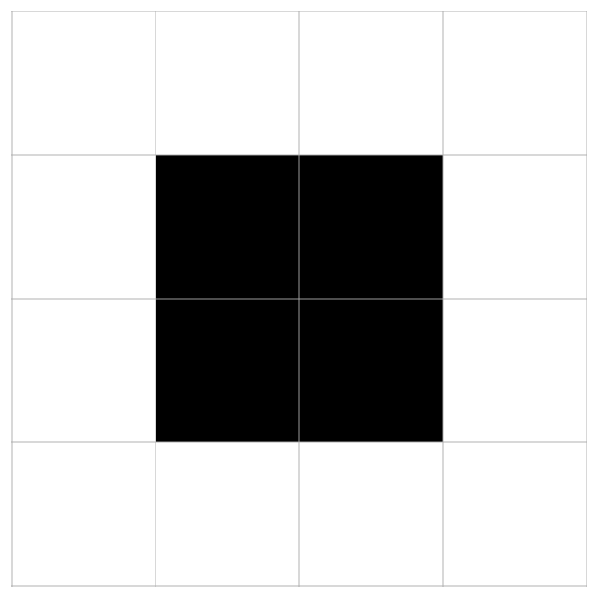
\includegraphics[width=\textwidth]{img/sl_block.png}
			\caption{\textit{Block}}
			\label{fig:block}
		\end{subfigure}
		\begin{subfigure}[b]{0.18\textwidth}
			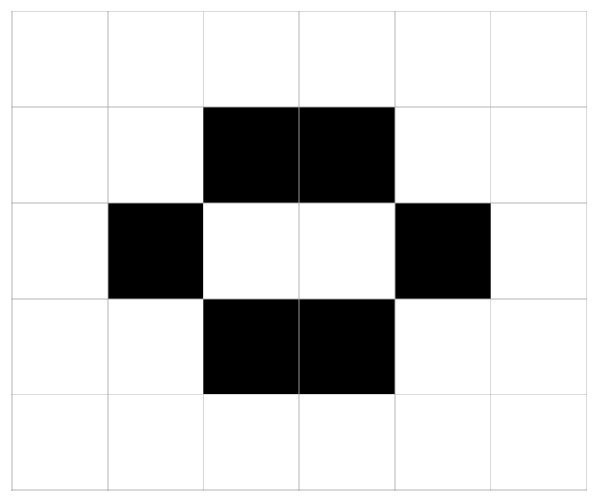
\includegraphics[width=\textwidth]{img/sl_beehive.png}
			\caption{\textit{Beehive}}
			\label{fig:beehive}
		\end{subfigure}
		\begin{subfigure}[b]{0.18\textwidth}
			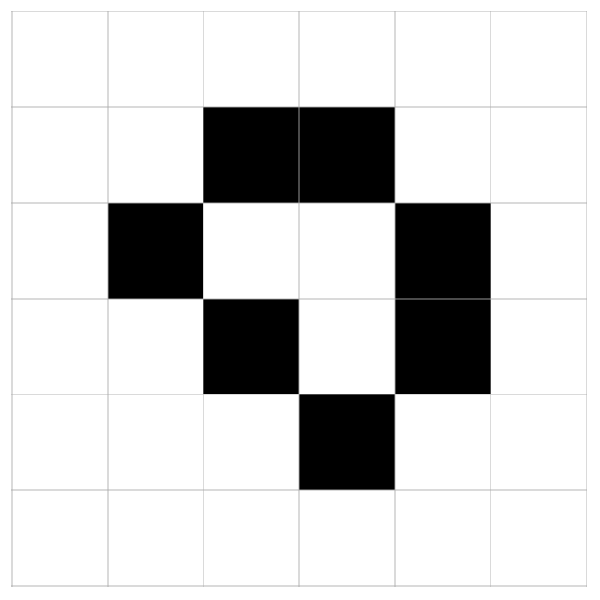
\includegraphics[width=\textwidth]{img/sl_loaf.png}
			\caption{\textit{Loaf}}
			\label{fig:loaf}
		\end{subfigure}
		\caption{Ejemplos de configuraciones de naturaleza muerta.}
		\label{fig:still_life}
	\end{figure}
	\item \textbf{Osciladores}: Patrones que repiten su configuración después de un número finito de iteraciones, manteniendo su posición en la cuadrícula.
	\begin{figure}[H]
		\centering
		\begin{subfigure}[b]{0.18\textwidth}
			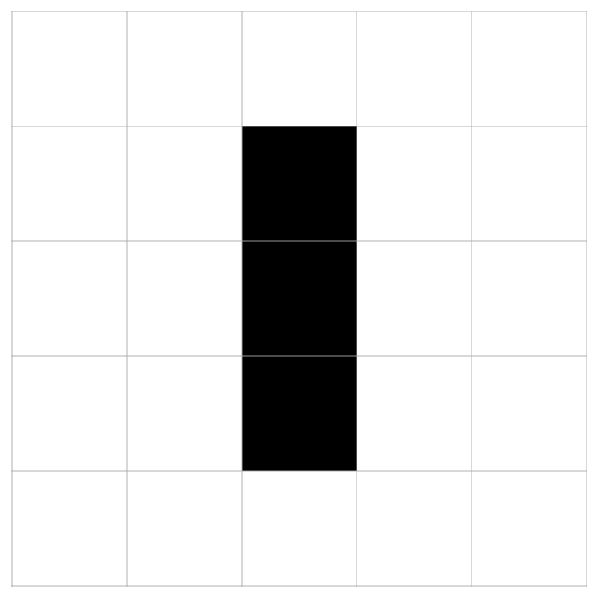
\includegraphics[width=\textwidth]{img/o_blinker_1.png}
		\end{subfigure}
		\begin{subfigure}[b]{0.18\textwidth}
			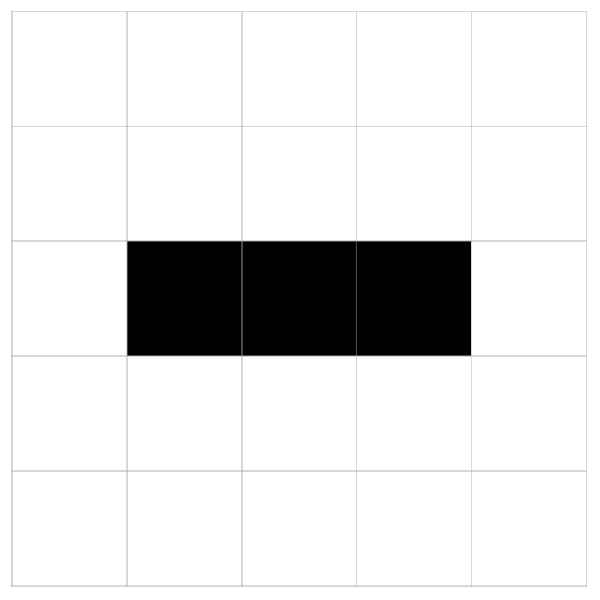
\includegraphics[width=\textwidth]{img/o_blinker_2.png}
		\end{subfigure}
		\caption{\textit{Blinker}.}
		\label{fig:blinker}
	\end{figure}
	\begin{figure}[H]
		\centering
		\begin{subfigure}[b]{0.18\textwidth}
			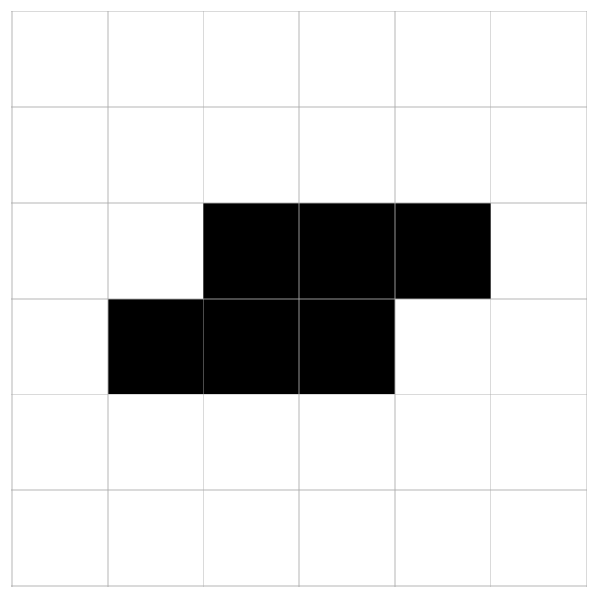
\includegraphics[width=\textwidth]{img/o_toad_1.png}
		\end{subfigure}
		\begin{subfigure}[b]{0.18\textwidth}
			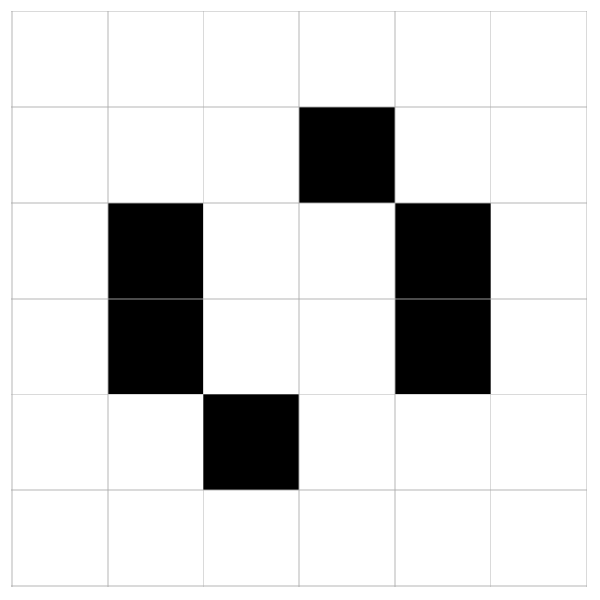
\includegraphics[width=\textwidth]{img/o_toad_2.png}
		\end{subfigure}
		\caption{\textit{Toad}.}
		\label{fig:toad}
	\end{figure}
	\item \textbf{Naves espaciales}: Son osciladores que, además de repetir su patrón, se desplazan por el espacio celular.  
	\begin{figure}[H]
		\centering
		\begin{subfigure}[b]{0.18\textwidth}
			
\includegraphics[width=\textwidth]{img/glider_1.png}
		\end{subfigure}
		\begin{subfigure}[b]{0.18\textwidth}
			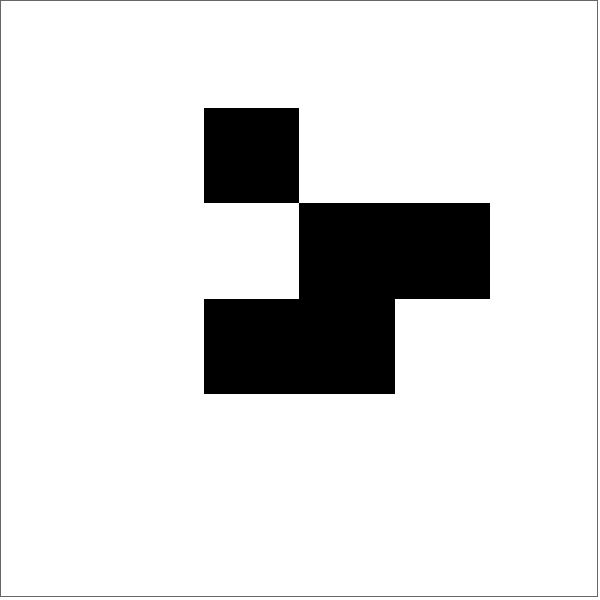
\includegraphics[width=\textwidth]{img/glider_2.png}
		\end{subfigure}
		\begin{subfigure}[b]{0.18\textwidth}
			
\includegraphics[width=\textwidth]{img/glider_3.png}
		\end{subfigure}
		\begin{subfigure}[b]{0.18\textwidth}
			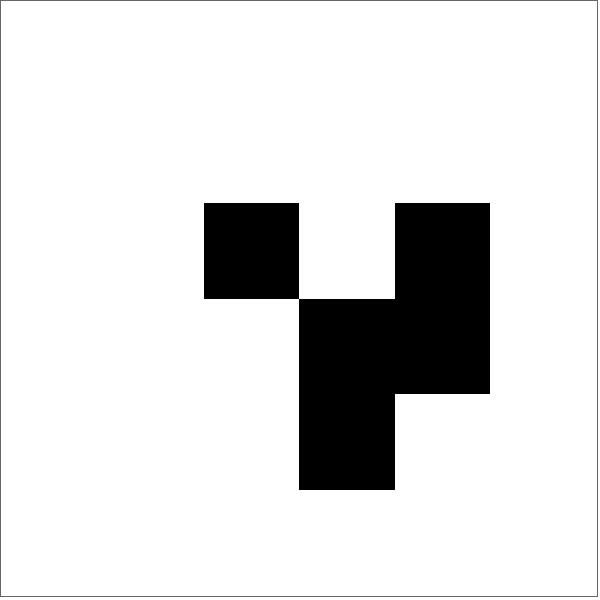
\includegraphics[width=\textwidth]{img/glider_4.png}
		\end{subfigure}
		\begin{subfigure}[b]{0.18\textwidth}
			
\includegraphics[width=\textwidth]{img/glider_5.png}
		\end{subfigure}
		\caption{\textit{Glider}.}
		\label{fig:glider}
	\end{figure}
\end{itemize}

Paul Rendell \cite{sipper2017_rendell_life} demostró que, a partir de una configuración inicial apropiada, el \textit{Juego de la Vida} es Turing completo, es decir, tiene la capacidad de realizar cualquier cálculo computable mediante la simulación de una máquina de Turing. La figura \ref{fig:conway_turing} muestra la configuración inicial del autómata celular diseñado por Paul Rendell.

\begin{figure}[!htbp]
	
	\centering
	
	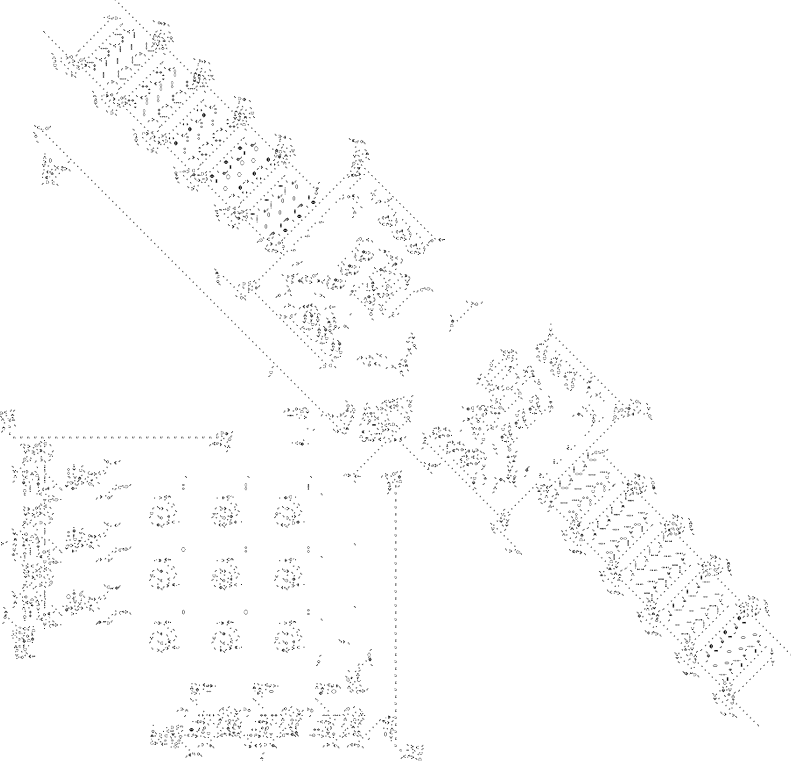
\includegraphics[width=0.85\textwidth]{img/gol_turing.png}
	
	\caption{Máquina de Turing implementada en el \textit{Juego de la Vida} \cite{rendell2000_turing_life}.}
	\label{fig:conway_turing}
\end{figure}

Debido a su naturaleza semitotalística, la vecindad puede dividirse en dos conjuntos, y con ello determinar el número de posibles estados que puede adoptar cada uno:

\begin{table}[!htbp] 
	
	\centering 
	
	\begin{tabular}{c|c|c}
		
		\hline \textbf{Vecindad} & \textbf{Estados} & \textbf{Total} \\ \hline 
		
		Frontera & $\{ 0,1,2,3,4,5,6,7,8 \}$ & 9 \\ 
		
		Centro & $\{ 0, 1 \}$ & 2 
		
	\end{tabular} 
	
\end{table}

Así, puede definirse un vector de 18 elementos que representa la función de transición, como se muestra en la tabla \ref{tab:life}.

\begin{table}[!htbp] 
	
	\centering 
	
	\begin{tabular}{c|c|c|c|c|c|c|c|c|c|c|c|c|c|c|c|c|c|c} 
		
		\hline 
		
		Frontera & 8& 7 & 6 & 5 & 4 & 3 & 2 & 1 & 0 & 8 &7 & 6 & 5 & 4 & 3 & 2 &1 &0 \\ 
		
		Centro & 1& 1& 1& 1& 1& 1& 1& 1& 1& 0& 0&0&0&0&0&0&0&0 \\ \hline 
		
		$B3/S23$ & 0 & 0 & 0 & 0 & 0 & 1 & 1 & 0 & 0 & 0 & 0 & 0 & 0 & 0 & 1 & 0 & 0 & 0 
		
		\\ \hline 
		
	\end{tabular}
	
	\caption{Representación binaria de la regla $B3/S23$.} 
	
	\label{tab:life} 
	
\end{table}

De manera general, el tamaño del vector que define una regla semitotalística puede calcularse mediante la ecuación \ref{eq:semitotalistica}. En este caso, dicho vector tiene tamaño 18, por lo que existen $|\mathcal{S}|^{18} = 2^{18} = 262,144$ posibles reglas.

\begin{equation}
	\prod_{i = 0}^{n} (|\mathcal{S}| - 1)(|n|) + 1, \quad \forall n \in \mathcal{N}
	\label{eq:semitotalistica}
\end{equation}

\subsection{Autómata celular elemental}

Stephen Wolfram propuso una versión más simple de los autómatas celulares, llamada autómata celular elemental. En esta versión, se disminuye la dimensionalidad del espacio celular y, por lo tanto, se reduce el tamaño de la vecindad. A continuación se detallan sus características según la definición formal de autómata celular:

\begin{itemize}
	
	\item \textbf{Espacio celular}: Está formado por una cadena unidimensional de celdas dispuestas linealmente.
	\item \textbf{Estados}: Cada célula puede encontrarse en uno de dos estados posibles, $\{0, 1\}$.
	\item \textbf{Vecindad}: Se define mediante un radio $r$ que determina cuántas celdas adyacentes influyen en la evolución de cada célula. En el caso del autómata celular elemental, el radio es $r = 1$, por lo que la vecindad está compuesta por la célula central y un vecino a cada lado.
	\item \textbf{Función de transición}: Wolfram no propuso una única regla de evolución, sino el conjunto completo de funciones de transición posibles bajo estas condiciones.
\end{itemize}

Dado que cada célula considera tres posiciones (la propia y sus dos vecinas) y cada una puede tener dos posibles estados, existen $2^3 = 8$ combinaciones de vecindad. Por tanto, el número total de reglas posibles es $2^{8} = 256$.

Wolfram asignó a cada una de estas funciones un número entero entre 0 y 255, conocido como número de regla, que identifica de forma unívoca el comportamiento del autómata. Además, propuso una clasificación de las reglas en cuatro categorías, según los patrones que emergen durante su evolución temporal (estas clases se detallan en la siguiente sección).

A continuación, se presentan tres reglas representativas por su relevancia teórica y sus propiedades computacionales.

\begin{itemize}
	
	\item \textbf{Regla 30}: La Regla 30 pertenece a la clase de comportamiento caótico. A partir de una configuración inicial simple, genera patrones altamente complejos y aparentemente aleatorios \cite{weisstein2002_rule30} como se muestra en las figuras \ref{fig:regla_30}.

	Esta regla plantea tres interrogantes fundamentales sobre la naturaleza del caos y la computabilidad:
	
	\begin{enumerate}
		\item ¿La columna central permanece no periódica a lo largo del tiempo?
		\item ¿Existe equilibrio estadístico entre los estados vivos y muertos?
		\item ¿Es posible calcular el estado de la célula central en el paso $n$ en tiempo $O(n)$?
	\end{enumerate}
	
	\begin{figure}[!htbp]
		\centering
		\begin{subfigure}[b]{0.75\textwidth}
			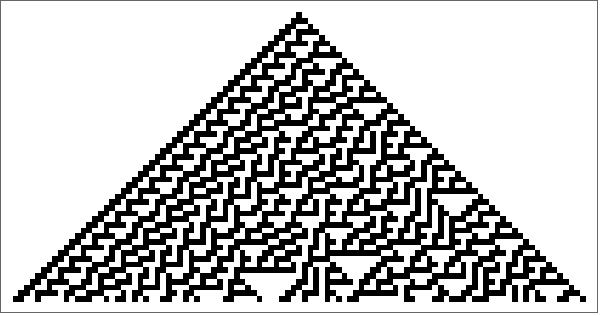
\includegraphics[width=\textwidth]{img/r30a.png}
			\caption{50 evoluciones.}
			\label{fig:30_1}
		\end{subfigure}
		\begin{subfigure}[b]{0.75\textwidth}
			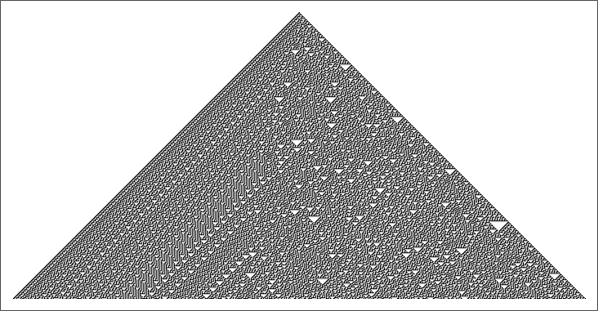
\includegraphics[width=\textwidth]{img/r30b.png}
			\caption{350 evoluciones.}
			\label{fig:30_2}
		\end{subfigure}
		\begin{subfigure}[b]{0.75\textwidth}
			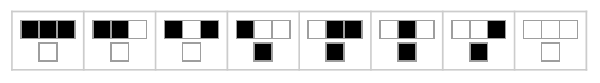
\includegraphics[width=\textwidth]{img/r30.png}
			\caption{Función de transición}
			\label{fig:30_rule}
		\end{subfigure}
		\caption{Evolución de la regla 30}
		\label{fig:regla_30}
	\end{figure}
	
	\item \textbf{Regla 110}: La Regla 110 exhibe un comportamiento mixto: combina regiones periódicas y caóticas que interactúan entre sí de manera compleja. A partir de una única célula activa, genera estructuras móviles y patrones que pueden coexistir en el tiempo \cite{weisstein2002_rule110}.
	
	Lo más notable de esta regla es su universalidad computacional. Wolfram y Matthew Cook demostraron que la Regla 110 es Turing completa, es decir, capaz de simular cualquier máquina de Turing y, por tanto, realizar cualquier cómputo posible en un sistema discreto determinista \cite{weisstein2002_rule110}. Su evolución se muestra en las figuras \ref{fig:regla_110}.
	
	\begin{figure}[!htbp]
		\centering
		\begin{subfigure}[b]{0.75\textwidth}
			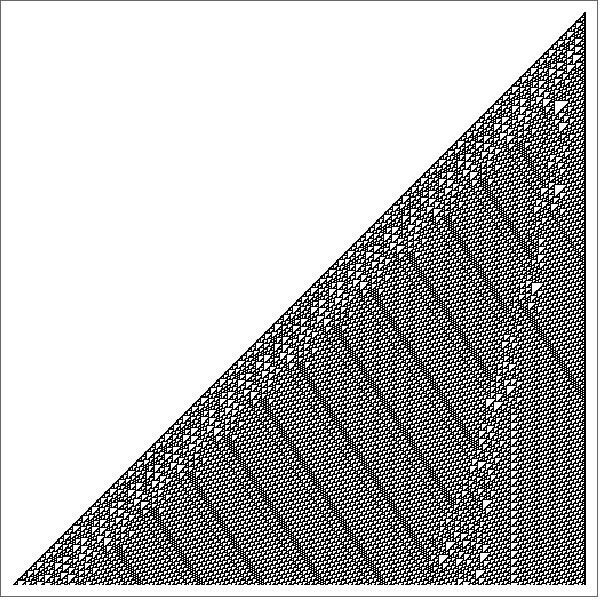
\includegraphics[width=\textwidth]{img/r110a.png}
			\caption{500 evoluciones.}
			\label{fig:110_1}
		\end{subfigure}
		\begin{subfigure}[b]{0.75\textwidth}
			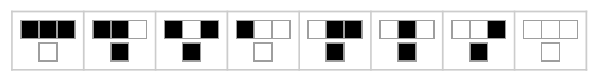
\includegraphics[width=\textwidth]{img/r110.png}
			\caption{Función de transición}
			\label{fig:110_rule}
		\end{subfigure}
		\caption{Evolución de la regla 110}
		\label{fig:regla_110}
	\end{figure}
	
	\item \textbf{Regla 90}: La Regla 90 se distingue por generar estructuras fractales. Iniciando desde una única célula activa, produce el conocido triángulo de Sierpinski como se muestra en la figura \ref{fig:regla_90}, el cual es un patrón autosimilar que aparece en múltiples sistemas naturales y matemáticos \cite{weisstein2002_rule90}.
	
	\begin{figure}[!htbp]
		\centering
		\begin{subfigure}[b]{0.75\textwidth}
			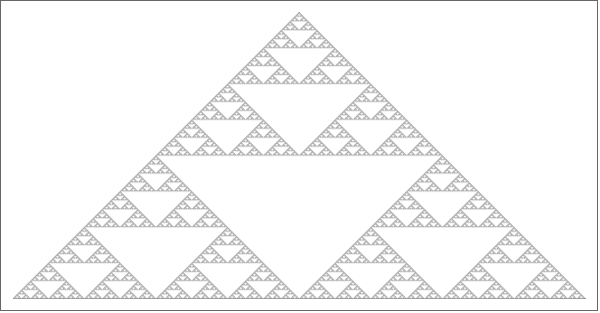
\includegraphics[width=\textwidth]{img/r90a.png}
			\caption{1025 evoluciones.}
			\label{fig:90_1}
		\end{subfigure}
		\begin{subfigure}[b]{0.75\textwidth}
			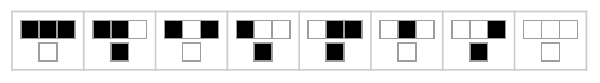
\includegraphics[width=\textwidth]{img/r90.png}
			\caption{Función de transición}
			\label{fig:90_rule}
		\end{subfigure}
		\caption{Evolución de la regla 90}
		\label{fig:regla_90}
	\end{figure}
\end{itemize}

\section{Clasificación}

Los autómatas celulares elementales fueron utilizados por diferentes autores por representar la máxima simplicidad y mínima configuración que un autómata puede adquirir y que tenga un amplio rango de comportamientos. Múltiples autores han intentado definir una clasificación; a continuación se muestran algunas clasificaciones propuestas por diferentes autores. 

Stephen Wolfram realiza una clasificación basada en el comportamiento que exhiben ciertas reglas y que es inherente a la configuración inicial. Es por esto que define las siguientes clases de comportamiento, ilustradas en la figura \ref{fig:clasificacion}:

\begin{enumerate}[label=W\Roman*]
	\item Evolucionan a un estado uniforme. 
	\item Evolucionan a estados cíclicos aislados.
	\item Evolucionan en comportamientos caóticos.
	\item Evolucionan en estados complejos aislados.
\end{enumerate}

\begin{figure}[!htbp]
	\centering
	\begin{subfigure}[b]{0.45\textwidth}
		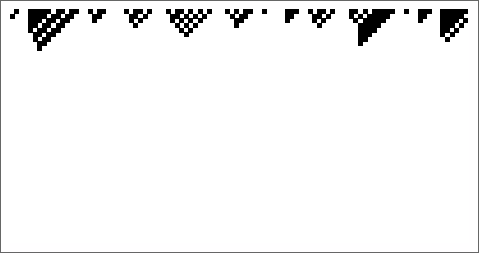
\includegraphics[width=\textwidth]{img/c1.png}
		\caption{Clase I: Regla 168}
		\label{fig:c1}
	\end{subfigure}
	\begin{subfigure}[b]{0.45\textwidth}
		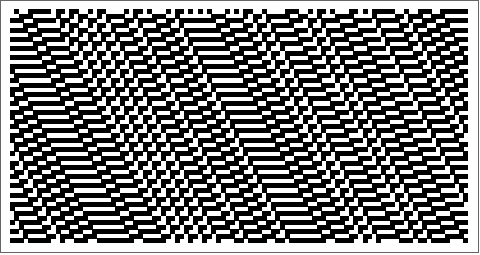
\includegraphics[width=\textwidth]{img/c2.png}
		\caption{Clase II: Regla 27}
		\label{fig:c2}
	\end{subfigure}
	\begin{subfigure}[b]{0.45\textwidth}
		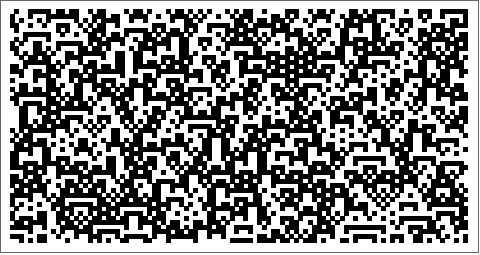
\includegraphics[width=\textwidth]{img/c3.png}
		\caption{Clase III: Regla 105}
		\label{fig:c3}
	\end{subfigure}
	\begin{subfigure}[b]{0.45\textwidth}
		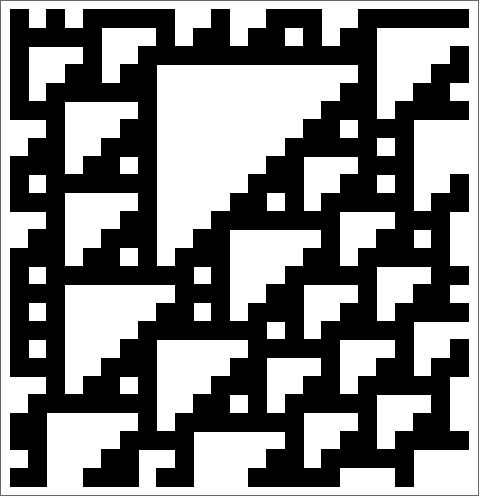
\includegraphics[width=\textwidth]{img/c4.png}
		\caption{Clase IV: Regla 106}
		\label{fig:c4}
	\end{subfigure}
	\caption{Clasificación de Wolfram. Las figuras evolucionan 50 pasos con la misma configuración inicial y con condición de frontera cíclica.}
	
	\label{fig:clasificacion}
	

\end{figure}

\begin{comment}
	
En la tabla \ref{tab:class_wolfram} se muestra la relación de reglas del autómata celular elemental. 

\begin{table}
	\centering
	\begin{tabular}{c|c|p{0.5\textwidth}}
		Tipo & Total & Reglas \\ \hline
		Clase I & 8 & 0, 8, 32, 40, 128, 136, 160, 168 \\ 
		Clase II & 65 & 1, 2, 3, 4, 5, 6, 7, 9, 10, 11, 12, 13, 14, 15, 19, 23,
		24, 25, 26, 27, 28, 29, 33, 34, 35, 36, 37, 38, 42,
		43, 44, 46, 50, 51, 56, 57, 58, 62, 72, 73, 74, 76,
		77, 78, 94, 104, 108, 130, 132, 134, 138, 140, 142,
		152, 154, 156, 162, 164, 170, 172, 178, 184, 200,
		204, 232. \\ 
		Clase III & 11 & 18, 22, 30, 45, 60, 90, 105, 122, 126, 146, 150. \\ 
		Clase IV & 4 &  41, 54, 106, 110.
	\end{tabular}
	\caption{Relación de reglas del autómata celular elemental con la clasificación de Wolfram.}
	\label{tab:class_wolfram}
\end{table}
\end{comment}

Sin embargo, existen reglas bajo diferentes configuraciones que pueden pertenecer a múltiples clases o, en el peor de los casos, no pertenecen a ninguna de ellas \cite{genaro2000_campo_promedio}. 

Li y Packard ofrecen otra clasificación que considera seis clases para categorizar el comportamiento dinámico de los autómatas celulares \cite{genaro2013_class}:
\begin{enumerate}[label*=LP\Roman*]
	\item La regla evoluciona a un estado homogéneo donde todas las células adquieren el mismo valor.
	\item Evoluciona hasta una configuración estática no necesariamente homogénea.
	\item Reglas con un periodo igual a dos.
	\item Reglas con un periodo de $L$.
	\item Evolucionan a estructuras caóticas.
	\item Conduce a estructuras largas y estructuras complejas.
\end{enumerate}

Por otro lado, Culick y Yu \cite{genaro2013_class, culik1988_class} proponen una clasificación que sigue las siguientes limitaciones: 

\begin{itemize}
	\item Esta clasificación es para autómatas celulares no totalísticos. 
	\item Cada clase es un subconjunto de la siguiente clase.
\end{itemize}

\begin{enumerate}[label*=CY \Roman*]
	\item Un autómata celular es de clase I si existe un estado estable $s \in \mathcal{S}$ tal que todas las configuraciones finitas evolucionan a una configuración homogénea de $s$.
	
	Es decir, dada cualquier configuración inicial en un autómata celular finito, todas las células adquieren el estado $s$ tras cierto número de pasos evolutivos. Esto se aplica a todas las finitas configuraciones iniciales.
	
	\item Un autómata celular es de clase II si existe un estado estable $s \in \mathcal{S}$ tal que se repite a $n$ pasos evolutivos.
	
	Esto implica que la evolución se repite cada $n$ número de pasos ($\sigma(t) = \sigma(t + n)$). Resulta evidente que la clase I está contenida en la clase II, haciendo que $n = 1$, lo que implica un periodo de uno.
	
	Una clasificación es $s$-finita si solo difiere del estado estable en una región finita.
	
	\item Un autómata celular es de clase III si existe un estado estable $s \in \mathcal{S}$ tal que para cualquier par de configuraciones $s$-finitas $C_1$ y $C_2$, es decidible si $C_1$ evoluciona a $C_2$.
	
	Es decir, si podemos determinar en tiempo finito si el CA evoluciona de $C_1$ a $C_2$, entonces pertenece a clase III. En caso contrario, pertenece a la clase IV, la cual contiene a todos los autómatas celulares \cite{culik1988_class}.
	
	\item Todos los autómatas celulares pertenecen a la clase IV.	
\end{enumerate}

\section{Extensiones y cambios de la definición}

Otra clasificación considera extensiones o modificaciones en la definición que alteran el comportamiento del autómata celular. A continuación, se describen algunas de estas extensiones para el modelado de sistemas complejos. 

\begin{itemize}
	
	\item \textbf{Autómatas celulares en grafos}: Amplían la idea de la estructura de red clásica al permitir que las vecindades no sean iguales: cada célula puede tener un número diferente de vecinos. Esta flexibilidad los hace adecuados para modelar fenómenos sobre grafos, como redes sociales o flujos en infraestructura. Sin embargo, diseñar manualmente las reglas de transición en estos entornos es una tarea compleja, lo que ha motivado propuestas como los autómatas celulares neuronales en grafos, que permiten aprender dichas reglas automáticamente \cite{grattarola2021_gca}.
	
	\item \textbf{Autómatas celulares probabilísticos}: Estos extienden el modelo clásico al incorporar reglas de transición estocásticas. En vez de una evolución que sigue un camino fijo, los estados futuros dependen de probabilidades que se ven afectadas por el entorno. Esto ayuda a entender la incertidumbre, el ruido y los comportamientos que surgen de manera inesperada. Son especialmente útiles para simular dinámicas como propagación de epidemias o sistemas sociales, donde los mecanismos de transición no siempre están completamente definidos \cite{gacs2024_pca}.
	
	\item \textbf{Autómatas celulares no homogéneos}: Permiten que diferentes células tengan diferentes funciones de transición. Para esto, se utilizan dos planos llamados ``plano de datos'', el cual contiene la evolución del sistema; y ``plano de control'', el cual define las reglas de transición para cada célula. Esto permite estudiar el comportamiento y la interacción entre diferentes reglas que comparten espacio \cite{hartman1987_ihca}.
	
	\item \textbf{Autómatas celulares continuos}: Son autómatas celulares que pueden ser continuos en los estados, en el tiempo y en el espacio \cite{Wolfram2002_nks}:
	
	\begin{itemize}
		\item Los estados continuos adquieren valores reales y no solo enteros.
		
		\item El tiempo continuo se define mediante una función que determina el intervalo de espera para actualizar la célula en función de su estado actual.
		
		\item El espacio continuo se obtiene al asignar diferentes pesos a las células dentro de la vecindad \cite{becker2023_cca}.
	\end{itemize}
\end{itemize}

Estas variantes no son exclusivas y además han ampliado el uso de los autómatas celulares. Sin embargo, un problema que se repite es definir correctamente las reglas de transición para lograr un fenómeno específico. Este desafío ha llevado a la creación de autómatas celulares neuronales. En estos, la función de transición no se define de manera clara, sino que se aprende a través de una red neuronal artificial. Pero antes de adentrarse en la definición, es necesario comprender qué son las redes neuronales.

\clearpage